% main.tex -- HistoAtlas, Research Article for Patterns (Cell Press)
% Source: arXiv preprint v1 (paper_workspace/arxiv_v1) and the v2 revision, re-checked
% against the frozen pipeline outputs. Figures: figures/*.pdf, rebuilt from
% figure_data/*.json by scripts/build_figures.py (see README.md).
% Class: elsarticle "review" mode -> single column, double spaced, line numbers,
% numbered references, which is the accepted Cell Press/Elsevier submission format.

\documentclass[preprint,review,12pt]{elsarticle}

\usepackage[T1]{fontenc}
\usepackage{lmodern}
\usepackage{amsmath,amssymb}
\usepackage{graphicx}
\usepackage{booktabs}
\usepackage{siunitx}
\usepackage{xcolor}
\usepackage[colorlinks=true,linkcolor=blue!60!black,citecolor=blue!60!black,
            urlcolor=blue!60!black]{hyperref}
\usepackage{microtype}
\usepackage{lineno}
\linenumbers

\graphicspath{{figures/}}
\sisetup{group-separator={,},group-minimum-digits=4}
\journal{Patterns}
\abstracttitle{Summary}

\newenvironment{hlbox}
  {\par\noindent\textbf{\large Highlights}\par\vspace{0.4em}
   \begin{itemize}\setlength{\itemsep}{0.2em}}
  {\end{itemize}\par\vspace{0.6em}}

\newsavebox{\bpbox}
\newenvironment{biggerpicture}
  {\setlength{\fboxsep}{10pt}%
   \begin{lrbox}{\bpbox}%
   \begin{minipage}{\dimexpr\textwidth-2\fboxsep-2\fboxrule\relax}%
   \textbf{\large The bigger picture}\par\vspace{0.5em}}
  {\end{minipage}\end{lrbox}%
   \par\vspace{0.8em}\noindent\fbox{\usebox{\bpbox}}\par\vspace{0.8em}}

\makeatletter
\def\ps@pprintTitle{\let\@oddhead\@empty\let\@evenhead\@empty
  \def\@oddfoot{\hfil\thepage\hfil}\let\@evenfoot\@oddfoot}
\makeatother

\begin{document}

\begin{frontmatter}

\title{HistoAtlas: an open, interpretable pan-cancer histomics resource
linking tissue morphology to molecular programs and clinical outcomes}

\author[1]{Pierre-Antoine Bannier\corref{cor1}}
\ead{pierreantoine.bannier@gmail.com}
\cortext[cor1]{Lead contact and corresponding author.}
\address[1]{Independent researcher}

\begin{abstract}
Routine hematoxylin-and-eosin pathology is the most widely collected tissue
assay in oncology, yet quantitative morphology is rarely released as reusable
data. HistoAtlas converts \num{6745} diagnostic whole-slide images from
\num{6088} patients across 21 cancer types into 38 named, compartment-resolved
morphological measurements and links each to survival, gene expression, copy
number, pathway activity and immune state, yielding \num{487638} precomputed
correlations and \num{5623} survival models reported with effect sizes,
confidence intervals and declared multiple-testing families. Six sparse
programs summarize the measurements. In \num{1095} slides from 817 patients
profiled by an independent consortium, the measurements and their
transcriptomic links transferred and extended to protein, with a narrow residual
that survives adjustment for matched transcripts. HistoAtlas is searchable
through a web atlas and a programmatic interface, and every statistic traces
back to tissue compartments and individual cells.
\end{abstract}

\begin{keyword}
computational pathology \sep histomics \sep pan-cancer atlas \sep
interpretable representations \sep multimodal data integration \sep
tumor microenvironment \sep external validation \sep FAIR data
\end{keyword}

\end{frontmatter}

\begin{hlbox}
\item 6,745 pathology slides become 38 named, compartment-resolved measurements
\item Morphology-molecule links replicate in 1,095 slides from a second consortium
\item Six sparse morphology programs map to pathways and to protein abundance
\item An open atlas exposes 487,638 precomputed correlations to people and agents
\end{hlbox}

\begin{biggerpicture}
Hematoxylin-and-eosin (H\&E) stained tissue sections are prepared for nearly
every solid tumor diagnosed, and public cohorts such as The Cancer Genome Atlas
pair these slides with genomic, transcriptomic and clinical data. The tissue
features a pathologist assesses, such as tumor content, the position of immune
cells relative to tumor epithelium, nuclear size and shape, or mitotic activity,
are nevertheless rarely recorded quantitatively. Without such measurements, slide
images cannot be analyzed jointly with molecular and clinical data using standard
statistical methods.

HistoAtlas defines 38 quantitative tissue measurements, each computed from
segmented tissue compartments and classified cells by a fixed formula with a
physical unit, and applies them to \num{6745} slides from 21 cancer types. Every
measurement is tested against survival, gene expression, copy number, pathway
activity and immune state within a single statistical framework: effect sizes with
bootstrap confidence intervals, false discovery rate control within declared
families of tests, minimum detectable effects at fixed power, and
proportional-hazards checks for survival models. Because each value is computed
from identified cells in identified tissue regions, any association can be
inspected at the level of the image tiles that produced it. The measurements and
their molecular associations were re-evaluated, without refitting, in an
independent cohort of \num{1095} slides, where most prespecified associations
replicated. The complete tables are released through a web atlas and a
programmatic interface, so that new hypotheses can be checked against existing
results without reprocessing the images. The same approach, in which expert
visual assessments are defined as explicit measurements, their uncertainty is
quantified and their transfer across cohorts is tested, could be applied to other
imaging data that are currently interpreted qualitatively by specialists.
\end{biggerpicture}

\clearpage

\section{Introduction}
\label{sec:intro}

Hematoxylin-and-eosin (H\&E) staining of tissue sections is the most widely used
assay in cancer medicine~\cite{bera2019}. Every diagnostic
slide records tissue composition, cell densities, nuclear morphology and the
spatial arrangement of tumor and microenvironmental
cells~\cite{gurcan2009, vanderlaak2021}. For genomics, transcriptomics and
proteomics, pan-cancer resources release standardized, queryable
tables~\cite{kandoth2013, hoadley2014, li2023cptac, corces2018}; no equivalent
resource exists for histopathology. Diagnostic slides are archived at scale, but
the quantities a pathologist assesses from them are rarely recorded as numerical
data.

Bulk molecular assays average over the whole sample and do not record the
spatial organization of the tissue. Yet the density of immune cells in the tumor
core and at the invasive margin is prognostic in several cancer
types~\cite{galon2006, fridman2012immune, pages2018}. Saltz et~al.\ showed that
deep learning applied to public pathology slides recovers tumor-infiltrating
lymphocyte density at pan-cancer scale~\cite{saltz2018til}, but a density
computed over the whole slide does not distinguish lymphocytes inside tumor
epithelium from lymphocytes confined to the surrounding stroma, the pattern that
defines immune exclusion. Existing public resources each cover part of the
problem: cBioPortal provides molecular and clinical tables without quantitative
morphology~\cite{cerami2012cbio}, the Cancer Imaging Archive provides images
without associated statistical analyses~\cite{clark2013tcia}, and the Human
Protein Atlas provides immunohistochemistry-based maps of individual
proteins~\cite{uhlen2015hpa, uhlen2017pathology}, which are not available for
routine H\&E slides.

Computational pathology has made the extraction of tissue features tractable.
Early morphometric studies linked handcrafted image features to outcome and
molecular alterations in single cancer types~\cite{beck2011, cooper2015, yu2016}; more recent systems
predict molecular alterations, expression programs and outcomes directly from
H\&E~\cite{coudray2018, schmauch2020he2rna, bannier2024}, as reviewed
in~\cite{echle2021}; and foundation models now produce tile-level embeddings
that can be aggregated to the slide
level~\cite{chen2024uni, vorontsov2024virchow, hoptimus0}. These results
show that H\&E images contain substantial biological information. Foundation-model
embeddings are information-dense representations that support many downstream
tasks, including mutation, biomarker and outcome
prediction~\cite{filiot2023phikon, filiot2024phikonv2, bannier2024, bannier2024her2},
but they are not interpretable: an individual coordinate does not
correspond to a defined tissue property, so an association found with an
embedding cannot be attributed to specific cells or tissue regions.
Interpretable feature sets have been proposed~\cite{diao2021hif, abel2024}, but
no pan-cancer set of interpretable measurements has been released together with
its molecular and clinical associations and evaluated in an independent cohort.

Image statistics depend on staining protocol, scanner, fixation and case
selection, so a measurement defined in one cohort can have a different
distribution, and a different relationship to molecular variables, in another.
Measurements and associations derived from The Cancer Genome Atlas (TCGA)
therefore need to be re-estimated on slides from other institutions. The Clinical
Proteomic Tumor Analysis Consortium (CPTAC) provides independent diagnostic slides
with matched transcriptomic and proteomic profiles across several cancer
types~\cite{li2023cptac}. This allows two tests: whether the measurement
distributions and their correlations with gene expression are reproduced in an
independent cohort, and whether the same correlations are observed at the
protein level.

Here we present HistoAtlas. From \num{6745} TCGA diagnostic slides from
\num{6088} patients spanning 21 solid-tumor types, we derive 38 interpretable,
compartment-resolved histomic measurements and compute their associations with
survival, gene expression, copy number, pathway activity and immune state,
reporting effect sizes, confidence intervals, minimum detectable effects and
explicitly declared multiple-testing families throughout. We show that the 38
measurements can be summarized by six continuous programs, each correlated with
specific MSigDB Hallmark pathways~\cite{liberzon2015}; that the measurement distributions, their
correlations with gene expression and two of the six programs are reproduced in
\num{1095} independent CPTAC slides; that the correlations with gene expression
are also observed at the protein level, with 132 measurement--protein
correlations remaining significant after adjustment for the matched transcript;
and that adding the measurements to survival models that already include
clinical covariates and matched transcripts slightly improves discrimination. The resource is released as an interactive atlas and
a programmatic interface, in which every reported statistic is linked to the
tissue compartments and individual cells from which it was computed.

\section{Results}
\label{sec:results}

\subsection{HistoAtlas turns routine pathology into a named, compartment-resolved measurement layer}
\label{sec:results:resource}

We built HistoAtlas from \num{6745} H\&E-stained diagnostic whole-slide images
from \num{6088} patients spanning 21 TCGA solid-tumor types
(Table~S1). Twelve further TCGA types were excluded because their dominant cell
morphologies fall outside the training domain of the cell detection model,
including lymphoid, glial, melanocytic, mesenchymal, neuroendocrine, renal
tubular and germ-cell tumors (Table~S2). Descriptive analyses of the measurement
space use every slide; all statistical associations use one representative slide
per patient, so that the 312 patients with several slides are not counted more
than once.

The pipeline converts each slide into quantitative morphology in two stages
(Figure~\ref{fig:fig1}A). A tissue model assigns every region to one of five
compartments (cancerous epithelium, stroma, necrosis, normal epithelium, blood);
tumor and stroma together account for more than 90\% of analyzed tissue area, so
downstream measurements can be expressed relative to biologically meaningful
territory rather than to whole-slide area. The HistoPLUS cell
model~\cite{adjadj2026histoplus}, which classifies cells into 13 types, then
detects individual cells, of which nine types are used here (tumor cell,
lymphocyte, fibroblast, plasmocyte, neutrophil, eosinophil, red blood cell,
apoptotic body, mitotic figure), more
than four billion cells across the cohort. Signed distance transforms from the
tumor boundary define spatial bands, so that a lymphocyte counted inside tumor
epithelium is not confused with one counted 150~\textmu m away in stroma. From
these maps we derived 38 histomic measurements in six groups: tissue composition
(3), cell densities (8), nuclear morphology and kinetics (7), spatial organization
(11), spatial heterogeneity (5) and cell-type ratios (4) (Table~S3).

Across 22 analysis cohorts (21 cancer types
plus a pan-cancer set) we fitted \num{5623} Cox proportional hazards models
(four endpoints, each under an unadjusted and a covariate-adjusted
specification), of which \num{5283} yielded valid estimates after
proportional-hazards screening, and computed \num{487638} Spearman correlations
against messenger RNA expression, pathway activity, copy number and immune
deconvolution scores. Benjamini--Hochberg correction was applied within declared,
non-overlapping families (150 for correlations, defined by cancer type, molecular
data type and model). At a false discovery rate of 0.05, 260 survival
associations and \num{88920} molecular correlations were significant
(\num{87217} of them involving the 38 measurements; the others involve three
quality-control variables released in the same table; Table~S8). Every association carries an effect size, a bootstrap 95\% confidence
interval, raw and adjusted $P$ values, a minimum detectable effect at 80\% power,
a proportional-hazards flag where applicable, and the identifier and size of its
correction family.

Pairwise Spearman
correlation across the 38 measurements resolves coherent modules: immune-density
measurements form a tight positive block, nuclear morphometry clusters
separately, and cross-module anticorrelations, such as between tumor area
fraction and the tumor--stroma interface measurements, delineate distinct axes
(Figure~\ref{fig:fig1}B). Principal component analysis gives an effective
dimensionality of 18 components at 90\% explained variance, so the layer is
compressible but not collinear. A UMAP embedding of all \num{6745} slides
recovers expected morphological neighborhoods, with breast, liver, thyroid and
endometrial carcinoma occupying distinct regions and squamous and adenocarcinoma
types interleaved in the center (Figure~\ref{fig:fig1}C). Unsupervised $K$-means
partitioning into ten pan-cancer clusters recovers groups whose cancer-type
composition and measurement profiles are interpretable without any molecular
input (Figure~\ref{fig:fig1}D,E), and which are enriched for distinct immune
subtypes and Hallmark pathway states when molecular annotation is subsequently
overlaid (Figure~S1). Two of these purely morphological groups separate
prognostically in Cox models stratified by cancer type, so the effects are not
restatements of tissue of origin: a low-proliferation cluster dominated by liver,
thyroid and adrenocortical carcinoma (C2) was associated with better overall
survival (HR $= 0.54$, 95\%~CI $[0.40, 0.73]$, $P_{\mathrm{adj}} = 6.3 \times
10^{-4}$; 516 patients in the cluster, 108 events), and a high-interface cluster
dominated by breast and prostate carcinoma (C8) with worse survival (HR $= 1.36$,
95\%~CI $[1.15, 1.62]$, $P_{\mathrm{adj}} = 1.8 \times 10^{-3}$; \num{1112}
patients, 214 events).

\subsection{Six continuous morphological programs summarize the measurement space}
\label{sec:results:programs}

We applied
sparse principal component analysis ($\alpha = 1.0$) to the 38 measurements
across \num{5371} TCGA patients with complete measurement vectors, yielding six
continuous programs, each loading on 29 to 33 measurements with a few dominant
ones (Figure~\ref{fig:fig2}A). Their biological identities were not assigned in
advance but read off from correlations with 50 MSigDB Hallmark pathway scores~\cite{liberzon2015}
(Figure~\ref{fig:fig2}C): program~1 correlates most strongly with
\textsc{allograft\_rejection} ($\rho = 0.59$, $n = \num{5371}$) and the
interferon-$\gamma$ response ($\rho = 0.51$), program~2 with
\textsc{estrogen\_response\_early} ($\rho = 0.44$) and
\textsc{epithelial\_mesenchymal\_transition} ($\rho = 0.41$), and program~3 with
\textsc{myc\_targets\_v1} and \textsc{g2m\_checkpoint} (both $\rho = 0.53$). We
therefore label them immune infiltration, stromal architecture, nuclear atypia
and proliferation, tumor density, myeloid inflammation and fibroblast biology.
The same correspondence is
visible at the level of individual measurements, where immune densities align
with immune pathway signatures, nuclear morphometry and mitotic index with cell
cycle and proliferation signatures, and stromal and interface measurements with
the epithelial--mesenchymal transition, angiogenesis and coagulation signatures
(Figure~S2A).

\subsection{Compartment-resolved immune topology is prognostic and molecularly anchored}
\label{sec:results:immune}

Tumor-infiltrating lymphocytes are conventionally scored in the stromal
compartment~\cite{salgado2015til}; HistoAtlas measures lymphocyte density
separately in tumor epithelium and in stroma. Intratumoral
lymphocyte density was associated with improved overall survival in the
pan-cancer adjusted model (hazard ratio [HR] $= 0.87$, 95\%~CI $[0.81, 0.93]$,
$P_{\mathrm{adj}} = 9.8 \times 10^{-4}$, $n = \num{4560}$, \num{1356} events),
with the strongest cancer-specific effects in breast carcinoma (HR $= 0.72$,
95\%~CI $[0.60, 0.88]$, $P_{\mathrm{adj}} = 0.018$, $n = 960$) and head-and-neck
squamous carcinoma (HR $= 0.74$, 95\%~CI $[0.63, 0.87]$,
$P_{\mathrm{adj}} = 3.9 \times 10^{-3}$, $n = 444$; Figure~\ref{fig:fig3}A,B).
Stromal lymphocyte density, measured on the same slides by the same model,
showed a weaker pan-cancer effect (HR $= 0.89$, 95\%~CI $[0.83, 0.97]$,
$P_{\mathrm{adj}} = 0.031$, $n = \num{4561}$) and no significant effect in breast
carcinoma (HR $= 0.93$, 95\%~CI $[0.77, 1.12]$, $P_{\mathrm{adj}} = 0.67$). The
two compartments therefore separate: localization within tumor epithelium, not
lymphocyte abundance alone, carries the stronger prognostic
signal, consistent with the prognostic value of immune-cell location reported in
colorectal cancer~\cite{galon2006, pages2018}. In most of the 18 cancer types with an
evaluable adjusted model the intervals are wide and include 1, which is the expected
behavior of small cohorts (Figure~S3B).

The same distinction appears in the molecular data. Tumor--lymphocyte
nearest-neighbor distance at the invasive front, a direct spatial measure of
immune exclusion~\cite{joyce2015exclusion}, was inversely associated with
\textit{CD8A} expression in breast carcinoma ($\rho = -0.53$, 95\%~CI
$[-0.58, -0.48]$, $P_{\mathrm{adj}} = 1.8 \times 10^{-68}$, $n = 958$;
Figure~\ref{fig:fig3}C), and the top gene correlates of intratumoral lymphocyte
density are dominated by T-cell, B-cell and checkpoint transcripts
(\textit{TIGIT}, \textit{CD3E}, \textit{CD3D}, \textit{CD79A}, \textit{PDCD1},
\textit{CD8A}, \textit{CTLA4}), with luminal markers (\textit{ESR1},
\textit{PGR}, \textit{CCND1}) among the strongest negative correlates
(Figure~\ref{fig:fig3}D).

\subsection{Named measurements recover proliferation, invasion and differentiation programs}
\label{sec:results:bridge}

In TCGA breast
carcinoma, mitotic index correlated with canonical cell-cycle regulators,
including \textit{CCNE1} ($\rho = 0.568$, 95\%~CI $[0.519, 0.617]$,
$P_{\mathrm{adj}} = 2.7 \times 10^{-80}$, $n = 958$), \textit{PLK1}
($\rho = 0.558$ $[0.510, 0.607]$, $P_{\mathrm{adj}} = 5.1 \times 10^{-77}$),
\textit{AURKA} ($\rho = 0.539$, $P_{\mathrm{adj}} = 4.7 \times 10^{-71}$),
\textit{CHEK1} ($\rho = 0.526$) and \textit{BIRC5} ($\rho = 0.520$; all
$P_{\mathrm{adj}} < 10^{-64}$). Invasion depth, defined as the 75th percentile of
tumor distance from the tissue boundary, aligned with an
epithelial--mesenchymal axis (\textit{ZEB1}: $\rho = 0.318$
$[0.262, 0.375]$, $P_{\mathrm{adj}} = 8.4 \times 10^{-23}$, $n = 957$;
\textit{ALDH1A1}: $\rho = 0.327$, $P_{\mathrm{adj}} = 3.8 \times 10^{-24}$).
Nuclear pleomorphism, the coefficient of variation of tumor nuclear area,
correlated positively with proliferation genes (\textit{PLK1}:
$\rho = 0.484$, $P_{\mathrm{adj}} = 1.4 \times 10^{-55}$) and negatively with
luminal differentiation markers (\textit{BCL2}: $\rho = -0.374$,
$P_{\mathrm{adj}} = 8.1 \times 10^{-32}$; \textit{ESR1}: $\rho = -0.358$,
$P_{\mathrm{adj}} = 4.4 \times 10^{-29}$). These correspondences restate, in
continuous and automatically measured form, relationships that underpin
histopathological grading~\cite{elston1991grading}. Their value here
is that they are computed identically on every slide in the atlas, so they can
be compared across 21 cancer types rather than asserted one tumor type at a time.
Across all molecular data types the coupling is strongest for expression and
pathway activity and weakest for copy number: 80\% of pan-cancer adjusted
expression correlations and 83\% of pathway correlations were significant,
against 52\% for copy number (Figure~S2B).

\subsection{The measurement layer and its molecular links transfer to an independent consortium}
\label{sec:results:transfer}

Portability was assessed on \num{1095} CPTAC slides from 817 patients across five
cancer types with TCGA counterparts: breast ($n = 198$ slides), lung
adenocarcinoma ($n = 240$), head-and-neck squamous carcinoma (390 slides from 112
patients), pancreatic adenocarcinoma ($n = 175$) and endometrial carcinoma
($n = 92$).

For each cancer type we computed the standardized difference between cohort
medians, in units of the TCGA standard deviation, for each measurement, with a
prespecified criterion of at least 31 of 38 measurements within one standard
deviation. Four of five types passed: lung adenocarcinoma and pancreatic
adenocarcinoma at 34/38 (89.5\%), head-and-neck at 32/38 (84.2\%) and breast at
31/38 (81.6\%); endometrial carcinoma narrowly missed at 30/38 (78.9\%), driven by
tissue-composition shifts in the smallest cohort ($n = 92$ versus $n = 459$ in
TCGA; Figure~\ref{fig:fig4}A; Table~S9). The inter-measurement correlation
geometry was preserved across cohorts (Pearson $r = 0.84$ over the 703
upper-triangle pairs, $P < 10^{-180}$; Table~S9), indicating that the 38
measurements span the same latent morphological space in independent tissue.

The morphology-to-transcriptome bridge replicated. All ten prespecified
histomic--molecular associations matched in direction and nine remained
significant after correction within the full CPTAC family of approximately
\num{24700} tests per model per cancer type, including mitotic index with
\textit{PLK1} in lung adenocarcinoma ($\rho = 0.505$,
$P_{\mathrm{adj}} = 5.0 \times 10^{-5}$), invasion depth with \textit{ZEB1} in
breast carcinoma ($\rho = 0.319$, $P_{\mathrm{adj}} = 4.6 \times 10^{-3}$) and
nuclear pleomorphism with \textit{ESR1} ($\rho = -0.389$,
$P_{\mathrm{adj}} = 2.7 \times 10^{-4}$) and \textit{BCL2}
($\rho = -0.416$, $P_{\mathrm{adj}} = 7.7 \times 10^{-5}$). Beyond the
prespecified set, effect sizes were concordant at scale. Across 750 matched
feature--gene--cancer triples drawn from each cohort's strongest correlates, the
two cohorts' Spearman coefficients correlated at Pearson $r = 0.787$ (95\%~CI
$[0.758, 0.813]$, $P = 4.0 \times 10^{-159}$), with mean $|\rho|$ modestly
attenuated in CPTAC (0.251 versus 0.301). Across all \num{25155} evaluable
measurement--gene pairs, most of which are near zero in both cohorts, the
correlation was $r = 0.56$ (Figure~\ref{fig:fig4}B), as expected when weak
associations are estimated in small cohorts.

Program transfer was mixed in an informative way. Projecting the six
TCGA-fitted programs into 297 CPTAC patients with complete measurement vectors,
two-sample Kolmogorov--Smirnov tests showed no significant distributional shift
for the immune program ($D = 0.072$, $P = 0.10$) or the fibroblast program
($D = 0.064$, $P = 0.19$), a borderline shift for the stromal program
($D = 0.096$, $P = 0.010$), and larger shifts for the remaining three
($D = 0.15$ to $0.34$, $P < 10^{-4}$; Figure~\ref{fig:fig2}B). The programs also
validated at the protein level: the immune program tracked CXCL9
($\rho = 0.85$), CD79A ($\rho = 0.82$) and CD3E ($\rho = 0.78$) protein
abundance, and the stromal program tracked ZEB1 ($\rho = 0.72$) and FN1
($\rho = 0.71$), across \num{2220} program--protein pairs in four cancer types
(Table~S10). By contrast, transferring the ten hard cluster labels by
nearest-centroid assignment reproduced pathway enrichment only weakly (Spearman
$\rho = 0.15$, $P = 1.4 \times 10^{-3}$ across 450 cluster--pathway pairs), with
three of nine evaluable clusters concordant ($\rho = 0.38$ to $0.51$) and two
inverted ($\rho = -0.59$ and $-0.65$; Figure~S4). Adjusted Rand index between
cluster labels and cancer type was low in both cohorts (0.14 in TCGA, 0.07 in
CPTAC), confirming that the clusters capture morphology beyond tissue of origin.

\subsection{The bridge extends to protein, and the information added beyond bulk omics is incremental}
\label{sec:results:protein}

CPTAC's matched proteomics allowed the bridge to be tested one layer further
out. Across \num{14687} measurement--gene pairs with both messenger RNA and protein
measured, the two modalities' coefficients correlated at $r = 0.63$
(Figure~\ref{fig:fig4}C). Among the 320 pairs significant in both, directional
concordance was 98.8\% (316/320, 95\%~CI $[96.8\%, 99.7\%]$), and the median
protein-minus-RNA difference in effect size was essentially zero
($\Delta\rho = -0.007$). Protein was therefore not globally stronger than RNA,
but it was specifically stronger for markers where post-translational biology
dominates: nuclear pleomorphism tracked ESR1 protein more closely than
\textit{ESR1} transcript in breast carcinoma ($\rho = -0.440$ versus $-0.389$),
consistent with estrogen receptor protein being the phenotypic determinant of
luminal differentiation~\cite{allison2020erpr}, and stromal
measurements tracked vimentin protein more closely than transcript
($\rho = 0.578$ versus $0.344$). Mitotic index tracked cell-cycle proteins in
lung adenocarcinoma (MKI67, CDK1, TOP2A, CHEK1, PLK1), and intratumoral lymphocyte
density tracked CD79A, CD3E, GZMA, PRF1, GZMB and IDO1 protein in breast
carcinoma. Of the four biological axes probed by this triangulation, proliferation markers
are supported in all four lines of evidence, immune and hormonal markers in three
or four, and epithelial--mesenchymal markers mainly in TCGA transcripts and CPTAC
protein (Figure~\ref{fig:fig4}D).

Because protein abundance is largely set by transcript abundance, we asked how
much of this signal is protein-specific. Partial Spearman correlations between
each measurement and each protein, adjusting for the matched transcript, left
132 of \num{14687} triplets significant after correction (0.9\%), 120 of them in
breast carcinoma, including stromal and DNA-repair markers such as VIM
(Figure~\ref{fig:fig5}C); 77\% of protein correlations retained more than half
their magnitude after adjustment. Immune proteins such as CD8A and GZMB were
largely absorbed.

The same question can be asked of the survival results, and gives a
correspondingly measured answer. For each of three measurements we refitted the
strongest clinical Cox model with matched molecular covariates added
(\textit{CD8A}, \textit{TIGIT}, immune subtype and leukocyte fraction for the
immune measurements; the \textsc{g2m\_checkpoint} score and \textit{MKI67} for
mitotic index; Figure~\ref{fig:fig5}A). The hazard ratio for intratumoral
lymphocyte density in head-and-neck carcinoma was essentially unchanged (0.76 to
0.72, still significant), whereas the hazard ratios for tumor--lymphocyte
distance in cervical carcinoma (1.34 to 1.18) and mitotic index in mesothelioma
(2.00 to 1.40) moved toward 1 and were no longer significant, so part of those
associations is carried by the matched transcripts. Adding a measurement to a clinical-plus-RNA model raised Harrell's
apparent (in-sample) concordance index by a median of $+0.0007$ to $+0.0027$ across the 18 evaluable
cancer types for the three pan-cancer measurements ($+0.0038$ for nuclear
pleomorphism, tested in breast carcinoma only), and the increment was positive in
only 50\% to 61\% of individual cancer types; in
breast carcinoma, the largest cohort, intratumoral lymphocyte density added
$+0.008$ over clinical covariates plus \textit{CD8A} (Figure~\ref{fig:fig5}B).

\subsection{Calibration and sensitivity analyses mark where the atlas is reliable}
\label{sec:results:calibration}

Because HistoAtlas is meant to be reused, we characterized where its outputs are
stable and where they are not. Under a permutation null in which molecular
labels were shuffled within cancer type and the full production correction
pipeline was re-run (100 permutations over the \num{39900} measurement $\times$
pathway $\times$ cancer-type tests), the mean null discovery rate was
$1 \times 10^{-6}$ against an observed rate of 26.7\%
(empirical $P = 0.0099$, the smallest attainable with 100 permutations), so the
discovery rate is not a trivial consequence of sample size. Replacing
Benjamini--Hochberg with the more conservative Benjamini--Yekutieli procedure,
which permits arbitrary dependence among tests, retained 68.1\% of significant
correlations and 54.0\% of significant survival associations under a single
pooled correction family (Table~S11).

Targeted sensitivity analyses locate the confounders that matter. Adjusting for
molecular subtype attenuated the leading histomic--molecular correlations by
4.3\% in median $|\rho|$ in breast carcinoma and 6.2\% in endometrial carcinoma,
but by 28\% in pancreatic adenocarcinoma, where immune subtype carries much more
of the signal (Table~S12). Adjusting survival models for leukocyte fraction did
not erase the leading prognostic associations; slightly more measurements reached
significance afterwards (28/179 versus 25/179), indicating that they are not
simply surrogates for immune content (Table~S13). Batch effects from tissue
source site were present but not dominant: pan-cancer variance decomposition
attributed 44.7\% of variance to source site, 32.7\% to cancer type and 22.6\% to
residual, while within the 20 cancer types with several sites, source site
accounted for a median of 21.3\%, and all per-cancer silhouette scores by source
site were negative (Figure~S3A). Statistical power is the binding constraint in
small cohorts: breast carcinoma can detect HR~$\geq 1.62$ at 80\% power, whereas
cholangiocarcinoma ($n = 36$) requires HR~$\geq 3.75$, which is why \num{4846} of
\num{5623} survival associations carry an \emph{insufficient} evidence badge
(Figure~S3B).

Some measurements are more protocol-sensitive than others. Median tumor nuclear
irregularity shifted systematically between cohorts in all five matched cancer
types (standardized difference 1.8 to 2.4 TCGA standard deviations, largest in
lung adenocarcinoma; Figure~\ref{fig:fig4}A), a scale of shift that would
distort any cross-cohort comparison of that measurement. The atlas flags it
accordingly. Taken together, these analyses argue that HistoAtlas should be
consumed as a calibrated resource rather than an undifferentiated catalog: the
measurement layer is portable, the continuous programs are more reliable
cross-cohort units than the hard clusters, and the strongest claims are those
supported simultaneously by TCGA discovery, CPTAC replication and sensitivity
analyses that bound the plausible confounders.

\subsection{An open atlas makes pan-cancer morphology reusable by people and by machines}
\label{sec:results:atlas}

The statistical layer described above is released, not summarized. HistoAtlas is
served as a static web application at
\href{https://histoatlas.com}{histoatlas.com}, backed by precomputed JSON so
that no analysis server is required at runtime, and as a machine-queryable
interface exposing 45 typed tools over the same tables. A user can enter from
any of four directions: a measurement (what does intratumoral lymphocyte density
predict, and where), a cancer type (which measurements matter here), a molecular
entity (which morphologies track \textit{ESR1}), or a slide (what does this case
look like relative to the cohort). Each association is displayed with its effect
size, confidence interval, adjusted $P$ value, evidence badge, minimum
detectable effect, correction-family size and proportional-hazards status, so
that a weak result is legible as weak rather than merely present. Measurement
tables, per-slide values, cluster assignments and the full association tables
are downloadable.

Selecting a survival association leads to the measurement's definition
(Figure~\ref{fig:fig6}), from
there to the per-slide compartment map on which it was computed, and from there
to the individual image tiles that contributed most to the value, overlaid with
the cell-level predictions that generated them. The contrast between
intratumoral and stromal lymphocyte density in breast carcinoma is, at the top
of the stack, two hazard ratios (Figure~\ref{fig:fig6}B); at the bottom it is
the tiles that drive each score on one slide (Figure~\ref{fig:fig6}C,D). The
same view also exposes what a number hides: the third-ranked intratumoral tile on
this slide is dominated by fibroblasts rather than lymphocytes, a case a user can
see, question and report. A user who distrusts a number can look at the cells
behind it, which is not possible for a resource built on learned embeddings.
The programmatic interface exposes the same objects as structured tool calls,
so the atlas can also be queried by automated agents conducting systematic
hypothesis generation rather than only by humans browsing pages.

\section{Discussion}
\label{sec:discussion}

HistoAtlas converts
routine H\&E pathology into 38 named, compartment-resolved measurements, attaches
a fully declared statistical layer to them, validates that layer in an
independent consortium, and publishes the result as queryable infrastructure with
provenance back to individual cells. The individual biological correspondences
reported here are, for the most part, expected.

What distinguishes this from another predictive computational-pathology system is
what the coordinates mean. Foundation-model embeddings are information-dense inputs for predictive
models~\cite{chen2024uni, vorontsov2024virchow}, but they are not interpretable:
their dimensions have no units,
cannot be compared between studies, and do not decompose into quantities a
pathologist can check, such as lymphocyte density inside tumor epithelium or
distance from a tumor cell to its nearest lymphocyte. Because HistoAtlas
measurements are named, they can be given confidence intervals that mean
something, corrected within families that can be audited, compared across
cohorts on their own scale, and traced back to the tissue that produced them. The cost is expressive
power: interpretable measurements will not match learned representations on pure
predictive benchmarks.

In the independent CPTAC cohort, the measurement distributions, the
correlations between measurements and the correlations with gene expression
were reproduced, two of six program distributions were unchanged, and
cluster-level pathway enrichment was not reproduced. At the measurement level, four of five matched cancer types passed the
prespecified concordance criterion and the inter-feature correlation geometry
was preserved, so the coordinates mean approximately the same thing on tissue
processed elsewhere. At the biological level, the strongest external evidence
came from molecular associations rather than from survival: all ten prespecified
histomic--transcriptomic associations replicated in direction and nine in
significance, effect sizes were concordant across 750 matched triples, and the
bridge extended to protein abundance with 98.8\% directional agreement among
doubly-significant pairs. Continuous programs transferred better than discrete
clusters, which is a useful negative result: it says that the reusable units of
this atlas are the measurements and their sparse combinations, not any
particular partition of feature space. Users should treat the ten-cluster
solution as a browsing convenience.

Several findings show what the layer is good for. The separation between
intratumoral and stromal lymphocyte density quantifies a compartment effect that
bulk tumor-infiltrating-lymphocyte scoring collapses~\cite{saltz2018til,
galon2006}; tumor--lymphocyte distance captures immune exclusion as a
geometric quantity rather than an impression; mitotic index tracks cell-cycle
transcripts and proteins; nuclear pleomorphism tracks luminal differentiation
markers, more closely at the protein level than at the transcript level, as
estrogen-receptor biology predicts. None of these is conceptually new. The
advance is that they are available systematically, pan-cancer, with units and
error bars, for anyone to query.

The proteomics analyses position the resource within the wider ecosystem. TCGA
anchored pan-cancer genomics and transcriptomics; CPTAC extended it to
proteomics~\cite{li2023cptac}; HistoAtlas adds morphology alongside them. The
finding that histomic measurements correlate coherently with protein abundance in
independent tissue argues that H\&E morphology is not merely a low-fidelity
shadow of RNA. But the stricter test constrains that claim sharply: after
adjustment for matched transcripts only 132 of \num{14687} feature--protein
triplets remained significant, concentrated in stromal and DNA-repair markers.
HistoAtlas is therefore not an alternative to transcriptomics or proteomics. It
is a widely available, spatially resolved, interpretable readout that tracks
many molecular states and adds a narrow increment beyond them. The survival
analyses point the same way: adding a measurement to a clinical-plus-RNA model
raised the apparent concordance index by a median of $+0.0007$ to $+0.0038$, with
gains in only about half of individual cancer types, and two of three prognostic
associations weakened toward the null once matched transcripts were added.

For researchers, the practical value is that a question requiring morphology can
now be asked without reprocessing images. A user can ask which measurements
associate with a given pathway in a given cancer type, compare a candidate
feature's behavior across 21 tumor types, check whether an association survives
subtype adjustment, or retrieve the minimum effect a given cohort could have
detected before concluding that a null result is informative. The atlas is also
available as a Model Context Protocol (MCP) server, which agentic systems can
query directly.

Several limitations bound what can be concluded. All associations are
observational and cross-sectional; none supports a causal claim. External
validation was substantially stronger for molecular associations than for
survival, because CPTAC follow-up was absent or minimal in the highest-priority
validation cohorts, so clinical-outcome claims rest primarily on TCGA. The
measurements inherit the errors of upstream segmentation: the cell model was
trained on eight cancer types, and 13 of the 21 included types were processed
out of distribution, with reduced detection sensitivity inflating kinetic indices
in some of them. Median tumor nuclear irregularity shifted by 1.8 to 2.4
standard deviations between cohorts and should not be compared across protocols.
Molecular subtype adjustment attenuated correlations by 28\% in pancreatic
adenocarcinoma against under 7\% in breast and endometrial carcinoma, so
subtype-aware reporting is needed in tumors with strong molecular substructure.
Cohort sizes are severely unequal, and 86\% of survival associations carry an
insufficient-evidence badge, reflecting power rather than absence of signal.
Molecular annotation is incomplete; analyzing one representative slide per
patient discards intra-patient heterogeneity, although the 312 TCGA patients
with several slides make it estimable in future releases; the nine-class taxonomy underlying the
measurements does not resolve macrophage or dendritic-cell populations that
matter for microenvironment biology, and the atlas has
not been benchmarked against foundation-model embeddings or against hybrid
representations that combine both.

Those limitations define the next steps: additional external cohorts to map
which measurements are protocol-robust, spatial transcriptomics as a stronger
ground truth for compartment-resolved immune and stromal quantities, prospective
and treatment-annotated cohorts to test clinical utility properly, and a direct
benchmark of interpretable measurements against learned embeddings to quantify
what interpretability costs. HistoAtlas as it stands is a reference layer: a
standardized, externally validated, openly queryable account of what routine
cancer pathology contains, built so that other people's questions can be asked
of it.

\section{Methods}
\label{sec:methods}

\subsection{Cohort construction}
\label{sec:methods:cohorts}

\paragraph{Discovery cohort (TCGA).}
Formalin-fixed, paraffin-embedded H\&E-stained diagnostic whole-slide images were
obtained from The Cancer Genome Atlas via the Genomic Data Commons portal for 21
solid-tumor types (Table~S1). Slides were excluded if viable tissue
area fell below 1~mm$^2$, if severe processing artifacts were present (pen marks
covering $>$20\% of tissue area, or out-of-focus regions), or if essential
clinical metadata (vital status, follow-up time) were missing, leaving
\num{6745} diagnostic slides from \num{6088} patients (312 patients contributed
more than one slide). Slide-level descriptive analyses (the inter-measurement
correlation geometry, the UMAP embedding and pan-cancer clustering) used all
\num{6745} slides. To avoid pseudo-replication, every statistical association
used one representative slide per patient, chosen by a deterministic priority
ranking (quality-control pass status, then tissue-area adequacy, then
tile-extraction coverage, then tile count, then slide name). Twelve further
TCGA cancer types were excluded in their entirety because their dominant cell
morphologies fall outside the training domain of the cell detection model
(Table~S2). GDC file UUIDs for all \num{6745} slides are listed in
the code repository.

Matched clinical data (overall, disease-specific, disease-free and
progression-free survival; age at diagnosis, sex, pathologic stage, tissue source
site and tumor purity) came from the TCGA Pan-Cancer Clinical Data
Resource~\cite{liu2018tcgacdr}. Molecular data comprised RNA-seq expression
(RSEM-normalized), somatic mutations from the MC3 multi-caller
ensemble~\cite{ellrott2018mc3}, copy-number variation, immune cell fractions from
CIBERSORT~\cite{newman2015cibersort} and xCell~\cite{aran2017xcell}, tumor purity
from ABSOLUTE~\cite{carter2012absolute}, and immune subtypes (C1--C6) from
Thorsson et~al.~\cite{thorsson2018immune}. Molecular data were matched to slides
by TCGA case barcode (first 12 characters); for patients with multiple aliquots
the primary-tumor aliquot was used. Of \num{6745} slides, \num{5590} (82.9\%) had
matched immune subtype labels.

\paragraph{Validation cohort (CPTAC).}
Diagnostic H\&E slides and matched transcriptomic, proteomic and clinical data
were obtained for five CPTAC cancer types with TCGA counterparts: breast
carcinoma (198 slides), lung adenocarcinoma (240), head-and-neck squamous
carcinoma (390 slides from 112 patients), pancreatic adenocarcinoma (175) and
endometrial carcinoma (92), totalling \num{1095} slides from 817 patients. The
identical pipeline, model weights and feature definitions used for TCGA were
applied without retraining, recalibration or cohort-specific tuning. For patients
with multiple slides, one representative slide was selected by a deterministic
priority ranking (quality-control pass status, then tissue-area adequacy, then
tile-extraction coverage, then tile count, then fewest missing measurements, then
slide name), and all downstream analyses were performed at patient level.
Global tandem-mass-tag proteomics were available for four of the five types
(head-and-neck squamous carcinoma is a GDC-only study without a proteomic
profile).

\subsection{Tissue segmentation}
\label{sec:methods:tissue}

Tissue segmentation used a CellViT-inspired architecture~\cite{hoerst2024cellvit}
with a Phikon self-supervised ViT-B backbone~\cite{filiot2023phikon}, trained on
the PanopTILs crowdsourced annotation dataset~\cite{liu2024panoptils}. Inference was performed at
0.5~\textmu m/px on $224 \times 224$~pixel tiles with 32-pixel overlap, with the
final mask obtained by majority voting in overlap regions. The model assigns nine
tissue classes (cancerous epithelium, stroma, necrosis, normal epithelium,
tumor-infiltrating lymphocytes, junk/debris, blood, other, whitespace); mean
intersection-over-union was 0.72 on the PanopTILs held-out test set, with
substantial per-class variation and near-zero recall for necrosis and normal
epithelium in deployment, reflecting their rarity in both the training set and
resected TCGA specimens. Following the International Immuno-Oncology Biomarker
Working Group recommendation~\cite{salgado2015til}, regions classified as
tumor-infiltrating lymphocytes were reassigned to stroma before all downstream
computation, yielding five effective compartments: cancerous epithelium, stroma,
necrosis, normal epithelium and blood.

\subsection{Cell segmentation and classification}
\label{sec:methods:cells}

Cell instance segmentation and classification used
HistoPLUS~\cite{adjadj2026histoplus}, which classifies cells into 13 types; the
nine used here are
tumor cells, lymphocytes, fibroblasts, plasmocytes, neutrophils, eosinophils,
red blood cells, apoptotic bodies and mitotic figures (mean panoptic quality
0.509; per-class 0.28 to 0.73, lowest for rare types). Inference used
$224 \times 224$~pixel tiles at 40$\times$ magnification (0.25~\textmu m/px) when
available, falling back to 20$\times$ (0.50~\textmu m/px); most slides were
scanned at 40$\times$. Tiles were extracted with a 64-pixel (16~\textmu m)
overlap margin and cells in overlap regions were deduplicated by a union-find
procedure merging instances whose centroids fall within 10~\textmu m, roughly the
diameter of an epithelial nucleus. The cell model was trained on pathologist
annotations from eight cancer types (LUAD, LUSC, BRCA, COAD, BLCA, OV, PAAD,
MESO); the remaining 13 included types were processed out of distribution.
Tissue--cell discordance (cells inside a tissue-model tumor region not classified
as tumor cells) ranged from 0\% to 12\% across cancer types, highest in
pancreatic adenocarcinoma (12.2\%) despite being in distribution, plausibly
because of dense desmoplastic stroma and small tumor glands; out-of-distribution
types additionally showed inflated kinetic indices in prostate, liver and thyroid
carcinoma attributable to reduced detection sensitivity. Red blood cells and
plasmocytes were not used in measurement computation.

\subsection{Spatial compartment definition}
\label{sec:methods:spatial}

All spatial computations were performed on compartment masks resampled to a
common 8~\textmu m/px grid by nearest-neighbor interpolation, so that boundary
quantities are scanner-invariant. Connected components below
$A_{\min} = \num{2048}$~\textmu m$^2$ were removed per compartment before
distance-transform computation, to prevent segmentation fragments from inflating
boundary lengths. Five spatial bands were defined from the signed Euclidean
distance transform $d_T$ to the tumor boundary (the outer contour of the
cancerous epithelium mask; positive inside tumor): tumor front
($0 \leq d_T \leq 50$~\textmu m), tumor core ($d_T > 50$~\textmu m), near stroma
($-50 \leq d_T < 0$), far stroma ($-200 \leq d_T < -50$) and necrosis ring
(within 100~\textmu m of the necrosis boundary). The 50~\textmu m front band
corresponds to approximately five cell diameters; the 200~\textmu m stromal
cutoff is a design parameter of the pipeline. Slides were assigned a growth-pattern
regime from the tumor front fraction
$\varphi = A(B_T^{0\text{-}50}) / A(\Omega_T)$: mass-forming
($\varphi \leq 0.5$), intermediate ($0.5 < \varphi \leq 0.8$) or infiltrative
($\varphi > 0.8$). Distance-based measurements are quantized at 8~\textmu m
owing to the grid spacing.

\subsection{Histomic measurement definitions}
\label{sec:methods:features}

We computed 38 quantitative histomic measurements per slide. For presentation
they are grouped into six categories: tissue composition (3), cell densities (8),
nuclear morphology and kinetics (7), spatial organization (11), spatial
heterogeneity (5) and cell-type ratios (4). The atlas's machine-readable feature
metadata uses a coarser five-way grouping of the same 38 measurements
(composition 3, density 6, morphology 8, spatial 18, heterogeneity 3); the two
schemes partition the identical set and no measurement differs between them.
Complete definitions, units and both category assignments are given in
Table~S3.

Two candidate measurements (normal epithelium area fraction and tumor--normal
contact fraction) were removed from the atlas entirely because the tissue model
did not reliably detect normal epithelium and both showed zero signal across all
slides. Seven ratio measurements were susceptible to unstable values when
denominators approach zero; these were controlled by winsorization
(\S\ref{sec:methods:preprocessing}).

\subsection{Measurement preprocessing}
\label{sec:methods:preprocessing}

Preprocessing proceeded in three steps. First, 22 measurements with heavy
right-skew (all densities, ratios, distances and heterogeneity measures) were
log-transformed as $\log(1 + x)$. Second, all 38 were winsorized at the 0.5th and
99.5th percentiles computed per measurement across the full cohort; global rather
than per-cancer percentiles were used because the target artifacts (segmentation
failures, ratio instabilities) occur across cancer types and because several
cohorts are too small (for example cholangiocarcinoma, $n = 38$) for reliable
percentile estimation. Third, measurements were $z$-score standardized. The scope
of standardization varied by analysis: UMAP and $K$-means used global $z$-scores;
Cox regression used per-cancer-type $z$-scores, so hazard ratios are per standard
deviation within cancer type; Spearman correlations used no standardization,
being rank-based. Missing values ($<$2\% of entries) were imputed with the
column median before standardization. Raw values are retained for display in the
web interface; all models consumed preprocessed values.

\subsection{Survival analysis}
\label{sec:methods:survival}

Associations between each measurement and four endpoints (overall survival,
designated primary; disease-specific, disease-free and progression-free survival)
were assessed by Cox proportional hazards regression using
\texttt{lifelines}~\cite{davidsonpilon2019} without penalization. Each model
tests a single measurement plus covariates; no multivariate models combining
several measurements are included in the atlas. Two specifications were fitted
per measurement, cancer type and endpoint: unadjusted (measurement only) and
adjusted (measurement, age at diagnosis, sex and pathologic stage, stratified by
tissue source site). Stratification lets each site carry its own baseline hazard
without consuming degrees of freedom, the standard approach for multi-center
data~\cite{therneau2000modeling}. Pan-cancer models additionally stratified on
cancer type, estimating one shared coefficient across per-type baseline hazards.
Hazard ratios are reported per one standard deviation of the preprocessed
measurement, with 95\% Wald confidence intervals from the observed Fisher
information.

For adjusted models, missing covariates were handled by multiple imputation by
chained equations (\texttt{scikit-learn} \texttt{IterativeImputer} with Bayesian
ridge, 5 imputations, maximum 10 iterations, seed incremented per imputation),
pooled by Rubin's rules, with the fraction of missing information recorded. When
covariate missingness exceeded 20\% in any variable, total sample size fell below
30, or fewer than 3 of 5 imputations converged, complete-case analysis was used
instead. Missingness arose mainly from incomplete staging (Table~S6). A minimum of $n \geq 30$ with $\geq$10 events was required, and models
were fitted only when residual degrees of freedom remained positive.

The proportional-hazards assumption was tested for every fitted model using
Schoenfeld residuals with the Kaplan--Meier time transform~\cite{grambsch1994},
flagged as pass ($P \geq 0.05$), warn ($0.01 \leq P < 0.05$) or fail
($P < 0.01$). When the assumption was violated ($P < 0.05$, covering both warn
and fail), the hazard ratio, confidence interval and $P$ value were invalidated,
and the $P$ value was set to 1.0 for correction so that family size is preserved
without inflating discoveries. Of \num{5623} fitted models, \num{5283} yielded
valid estimates. Restricted mean survival time (RMST) differences were computed
as an assumption-free complement, as the area under the Kaplan--Meier curve to a
cancer-type-specific horizon (default \num{1095}~days; 2~years for pancreatic
adenocarcinoma and mesothelioma; 5~years for thyroid and prostate carcinoma;
Table~S7) with Irwin variance~\cite{irwin1949}, tested by
\num{5000}-permutation inference on median-split groups with \num{1000}-resample
percentile bootstrap intervals, requiring $n \geq 20$ with $\geq$5 per group. We
note that dichotomization for RMST discards information relative to continuous
methods~\cite{royston2006}. Cluster-level survival used two-sided log-rank tests
of members against non-members.

\subsection{Molecular correlations}
\label{sec:methods:correlations}

Spearman rank correlations were computed between each of the 38 measurements and
322 molecular targets: 133 curated genes drawn from OncoKB~\cite{oncokb} and the
COSMIC Cancer Gene Census~\cite{sondka2018cgc}, immune checkpoint targets and
EMT/stemness markers~\cite{nieto2016emt} (Table~S4), each assessed
for expression and copy number ($133 \times 2$); the 50 MSigDB Hallmark pathway
scores~\cite{liberzon2015}; and 6
CIBERSORT immune cell fraction scores. Pathway activity was computed by
single-sample gene set enrichment analysis (\texttt{gseapy}
1.1.12)~\cite{barbie2009ssgsea, fang2023gseapy} on the batch-corrected TCGA Pan-Cancer expression
matrix from UCSC Xena~\cite{goldman2020xena}, excluding gene sets with fewer than
10 genes present after intersection.

Unadjusted models used \texttt{scipy.stats.spearmanr} with analytical
$t$-approximation $P$ values, chosen over permutation to avoid $P$-value banding,
with 95\% percentile bootstrap intervals from \num{1000} resamples.
Covariate-adjusted models used partial Spearman correlations computed by
rank-transforming measurement, target and covariates, residualizing the ranked
measurement and target against ranked covariates by ordinary least squares, and
correlating the residuals~\cite{conover1999}; $P$ values used the standard
partial-correlation $t$ statistic with $\mathrm{df} = n - 2 - k$ for $k$
one-hot-encoded covariate columns. Tissue source site entered as a grouped
covariate (five most frequent sites per cancer type, remainder collapsed to
``Other'') rather than a stratification variable, since rank residualization
requires explicit columns. A cancer type was analyzed if $n \geq 30$; each pair
required $n \geq 10$ non-missing observations. Per-task random seeds were derived
deterministically from a hash of the cancer type and feature names. The analysis
comprised \num{487638} evaluable pairs (measurements $\times$ 322 targets
$\times$ 22 cohorts $\times$ 2 models, excluding combinations with insufficient
data). Of these, \num{461130} involve the 38 measurements; the remaining
\num{26508} involve three slide-level quality-control variables (missingness
flag, number of missing measurements and number of outlying measurements) that
were computed alongside the measurements, are released in the same table, and
entered the same correction families.

\subsection{Categorical associations}
\label{sec:methods:categorical}

Associations with categorical molecular variables (somatic mutation status,
copy-number alteration, immune subtype) were tested per cancer type. Unadjusted
two-group comparisons used the two-sided Mann--Whitney $U$ test with Cliff's
$\delta$ as effect size, computed as the mean of $\mathrm{sign}(x_i - y_j)$ over
all pairs with \num{1000}-resample bootstrap intervals (bootstrap rather than
analytical intervals because ties violate the continuity assumption of the
analytical variance formula~\cite{cliff1993}). Variables with more than two
levels used the Kruskal--Wallis $H$ test with
$\eta^2_H = (H - k + 1)/(N - k)$~\cite{tomczak2014}, floored at zero.
Covariate-adjusted models used rank-ANCOVA with Freedman--Lane permutation
inference~\cite{freedmanlane1983} (\num{1000} permutations of covariate-only
residuals), with partial $\eta^2$ as effect size. Group ordering followed a fixed
convention (mutant before wild-type, altered before neutral) so that the sign of
Cliff's $\delta$ is interpretable across analyses. A minimum of $n \geq 30$ total
and $\geq$5 per group was required.

\subsection{Clustering and embedding}
\label{sec:methods:clustering}

Unsupervised clustering was performed at two levels. At the pan-cancer (L1)
level, all \num{6745} slides were clustered on the full 38-dimensional
preprocessed vector; at the cancer-specific (L2) level, clustering was performed
within each cancer type using cancer-type-specific $z$-scores. We used $K$-means
(\texttt{scikit-learn}, $n_{\mathrm{init}} = 10$, random state 42). For L1,
solutions were computed for $K \in \{3, \ldots, 25\}$ and scored by silhouette,
Calinski--Harabasz, Davies--Bouldin and gap statistics; $K = 10$ was selected on
convergence of silhouette (local maximum), Calinski--Harabasz (plateau) and
Davies--Bouldin (local minimum), the gap statistic favouring $K = 8$. No
dimensionality reduction was applied before clustering, to keep cluster feature
profiles interpretable; the effective dimensionality of 18 components at 90\%
explained variance implies moderate redundancy, which gives correlated
measurements proportionally more weight. For L2, $K$ was selected by the elbow
method over $K \in [2, 8]$~\cite{thorndike1953}, yielding 69 subclusters; cancer
types with fewer than 20 samples received a single cluster and individual
clusters with fewer than 10 samples were dropped. Stability was assessed by 50
iterations of 80\% subsampling without replacement, re-clustering and comparing
to the original labels by adjusted Rand index and mean best-match Jaccard
index~\cite{hennig2007}. Cluster names were generated from a fixed schema
combining an immune axis label, a stromal axis label, the most extreme remaining
measurement, and a cancer-enrichment tag where one type constitutes $\geq$40\% of
the cluster. Two-dimensional visualization used UMAP
($n_{\mathrm{neighbors}} = 15$, $\mathrm{min\_dist} = 0.1$, Euclidean, random
state 42)~\cite{mcinnes2018} for display only; no inference was drawn from
embedding coordinates and all clustering was performed in the original
38-dimensional space.

\subsection{Continuous histomic programs}
\label{sec:methods:programs}

Sparse principal component analysis (\texttt{scikit-learn} \texttt{SparsePCA},
6 components, $\alpha = 1.0$, random state 42) was fitted on standardized
measurements from \num{5371} TCGA patients with complete feature vectors, after
representative-slide selection. Programs were named automatically from their
top-three loading measurements and interpreted post hoc by Spearman correlation
against all 50 Hallmark pathway scores in TCGA. The fitted scaler and
decomposition were then applied unchanged to 297 CPTAC patients with complete
feature vectors. Distributional transfer was assessed by two-sample
Kolmogorov--Smirnov tests between TCGA and CPTAC program scores. Program--protein
associations were computed as Spearman correlations against CPTAC tandem-mass-tag
protein abundance (\num{2220} program--protein pairs across four cancer types).

\subsection{External validation in CPTAC}
\label{sec:methods:validation}

\paragraph{Measurement concordance.}
For each matched cancer-type pair we computed the standardized difference
$d = (\mathrm{median}_{\mathrm{CPTAC}} - \mathrm{median}_{\mathrm{TCGA}}) /
\mathrm{SD}_{\mathrm{TCGA}}$ per measurement over all slides of that type in each
cohort (Figure~\ref{fig:fig4}A shows the signed value). A measurement passes at
$|d| \leq 1.0$; a cancer type passes when more than 80\% of measurements
($\geq 31/38$) pass. The inter-measurement correlation geometry was compared by
computing the full $38 \times 38$ Spearman matrix separately in each cohort and
correlating the flattened upper triangles (703 pairs) by Pearson correlation,
with a prespecified pass criterion of $r > 0.80$.

\paragraph{Association replication.}
Ten histomic--molecular associations were prespecified from the TCGA analysis
before CPTAC results were examined. Their CPTAC $P$ values were corrected within
the full CPTAC correction family (approximately \num{24700} expression tests per
model per cancer type), not within the prespecified subset, so replication is
assessed against the same multiplicity burden as discovery. Direction
concordance and significance replication are reported with 95\% Clopper--Pearson
exact binomial intervals. Aggregate transfer was quantified by extracting the top
50 correlated genes per measurement per cohort for 8 representative measurements
across 4 matched cancer types, matching by gene symbol, and correlating the two
cohorts' Spearman coefficients across the resulting 750 triples by Pearson
correlation with Fisher $z$-transform intervals.

\paragraph{Survival replication.}
Eight prespecified survival hypotheses were tested. Following ICH E9 guidance for
confirmatory tests of prespecified hypotheses, nominal (uncorrected) $P$ values
are reported and no false-discovery correction was applied. Direction concordance
is computed only over associations that were significant in TCGA and for which
CPTAC had sufficient follow-up. Survival follow-up was absent or minimal in
breast (0 patients with overall survival data), lung adenocarcinoma (25) and
endometrial carcinoma (8), leaving pancreatic adenocarcinoma ($n = 110$) and
head-and-neck squamous carcinoma ($n = 41$) as the only evaluable cohorts; their
minimum detectable effects at 80\% power are HR~$\geq 1.71$ and HR~$\geq 2.45$
respectively, so this analysis is reported as underpowered by construction.

\paragraph{Cluster-structure transfer.}
A \texttt{StandardScaler} and $K$-means model ($K = 10$) fitted on TCGA were
applied unchanged to CPTAC by nearest-centroid prediction. Per-cluster pathway
enrichment (Cliff's $\delta$ from Mann--Whitney $U$ tests, in-cluster versus
out-of-cluster) was computed independently in each cohort and compared by
Spearman correlation, both per cluster and across all 450 matched
cluster--pathway pairs. Adjusted Rand index, normalized mutual information and
V-measure between cluster labels and cancer type were computed in both cohorts.

\subsection{Proteomics and protein-specific signal}
\label{sec:methods:proteomics}

Spearman correlations were computed between each measurement and CPTAC global
tandem-mass-tag protein abundance in the four cancer types with proteomic
profiles. Direction concordance between messenger RNA and protein was assessed
over pairs significant in both modalities after correction, with
Clopper--Pearson intervals. To determine how much of the protein signal is
independent of transcript abundance, we computed partial Spearman correlations
between each measurement and each protein adjusting for the matched transcript,
using the same rank-residualization procedure as
\S\ref{sec:methods:correlations}, over \num{14687} (measurement, gene, cancer
type) triplets, with Benjamini--Hochberg correction applied per cancer type.
Retention was summarized as the fraction of triplets for which the partial
coefficient retained more than half the magnitude of the unadjusted coefficient.

\subsection{Added-value analyses}
\label{sec:methods:addedvalue}

To test whether measurements carry information beyond bulk transcriptomics, Cox
models for four target measurements were refitted with matched molecular
covariates added to the clinical specification: \textit{CD8A}, \textit{TIGIT},
immune subtype and leukocyte fraction for intratumoral lymphocyte density and
tumor--lymphocyte nearest-neighbor distance;
\textsc{hallmark\_g2m\_checkpoint} and \textit{MKI67} for mitotic index; and
\textit{ESR1} plus PAM50 subtype for nuclear pleomorphism in breast carcinoma.
Incremental discrimination was quantified as Harrell's concordance index for four
nested models per cancer type (clinical only; clinical + RNA; clinical +
histomics; clinical + RNA + histomics), summarized as the median across the 18
cancer types with evaluable models, together with the fraction of cancer types in
which the increment was positive. Concordance was evaluated on the data used for
fitting, so the increments are apparent rather than cross-validated and are an
upper bound on out-of-sample gain.

\subsection{Multiple testing correction}
\label{sec:methods:multiple}

All $P$ values were corrected by the Benjamini--Hochberg
procedure~\cite{benjamini1995} within explicitly declared families, chosen to
pool biologically coherent tests without the conservatism of pooling unrelated
analyses (Table~S5 gives every family definition). Survival
families were defined per cancer type $\times$ endpoint $\times$ model, so that
correction pools only the 38 measurement-level tests within one biological
context; correlation families were defined per cancer type $\times$ molecular
data type $\times$ model, giving 150 families. Every adjusted $P$ value is stored
alongside its correction-family identifier and family size, so that any reported
result can be re-derived. Gene set enrichment analysis used its own canonical
false-discovery procedure based on pooled null normalized enrichment score
distributions~\cite{subramanian2005} rather than Benjamini--Hochberg. Overall
survival is the primary endpoint; the other three are sensitivity analyses,
corrected independently per endpoint rather than pooled, because the endpoints
share events and therefore violate the independence assumption of joint
correction. Permutation $P$ values used the add-one correction of Phipson and
Smyth~\cite{phipson2010permutation}. Bootstrap intervals used \num{1000}
percentile resamples and were reported only when $\geq$90\% of resamples produced
valid estimates. Unless stated otherwise, ``significant'' means
$P_{\mathrm{adj}} < 0.05$.

\subsection{Power analysis and evidence grading}
\label{sec:methods:power}

The minimum detectable effect size at 80\% power ($\alpha = 0.05$, two-sided) was
computed for every association: by the Schoenfeld--Freedman
approximation~\cite{schoenfeld1983, freedman1982} for survival, the Fisher
$z$-transform for correlations, and simulation-based power curves (\num{2000}
simulated datasets with binary search) for categorical associations. Every
association carries an evidence badge: \textbf{strong} ($P_{\mathrm{adj}} <
0.01$, effect above the medium-effect threshold, narrow interval, $n \geq 100$),
\textbf{moderate} ($P_{\mathrm{adj}} < 0.05$, effect above the small-effect
threshold, narrow or moderate interval, $n \geq 50$), \textbf{suggestive}
($P_{\mathrm{adj}} < 0.10$ or interval excluding the null, $n \geq 30$) or
\textbf{insufficient} ($n < 30$ or missing statistics). Thresholds for $\rho$ and $\eta^2$ follow
Cohen~\cite{cohen1988}, those for Cliff's $\delta$ approximate Romano
et~al.~\cite{romano2006}, and those for hazard ratios were set for this study:
medium, HR~$\geq 1.5$ or
$\leq 0.667$, $|\rho| \geq 0.3$, $|\delta| \geq 0.3$, $\eta^2 \geq 0.06$; small,
HR~$\geq 1.18$ or $\leq 0.847$, $|\rho| \geq 0.1$, $|\delta| \geq 0.15$,
$\eta^2 \geq 0.01$.

\subsection{Quality control, batch effects and sensitivity analyses}
\label{sec:methods:qc}

Batch effects from tissue source site were assessed by principal variance
component analysis~\cite{li2009pvca}, decomposing variance in the top principal
components (explaining $\geq$80\% cumulative variance, up to 10 components) into
site, cancer type and residual fractions using marginal one-way ANOVA $\eta^2$
weighted by explained variance. Because site and cancer type are not orthogonal,
marginal $\eta^2$ values can exceed 1.0 in sum; residual variance was computed as
$\max(0, 1 - \eta^2_{\mathrm{batch}} - \eta^2_{\mathrm{bio}})$ and all three
fractions renormalized. Silhouette analysis treated site labels as cluster
assignments on standardized measurements (Euclidean, subsampled to \num{5000}
slides), with scores above 0.25 flagged as moderate and above 0.5 as strong batch
effects.

Four sensitivity analyses were run. (i) A permutation null shuffled molecular
labels within cancer type and re-ran the full production correction pipeline over
the \num{39900} measurement $\times$ pathway $\times$ cancer-type tests for 100
permutations. (ii) The Benjamini--Yekutieli procedure, valid under arbitrary
dependence, was substituted for Benjamini--Hochberg; for this comparison all
tests of a given analysis type were pooled into a single family, so its
denominator (272 significant survival associations) differs from the production
149-family design (260). (iii) Top correlations were recomputed with molecular
subtype as an additional covariate (PAM50 for breast, molecular class for
endometrial, immune subtype for pancreatic carcinoma; the lung adenocarcinoma
driver stratification was uninformative because neither \textit{EGFR} nor
\textit{KRAS} mutation was prevalent enough to form contrasting groups).
(iv) Survival models for the top 10 measurements were refitted with leukocyte
fraction as an additional covariate.

\subsection{Software, reproducibility and interfaces}
\label{sec:methods:software}

All analyses were implemented in Python 3.11 and orchestrated as a directed
acyclic graph by Snakemake~\cite{moeldner2021snakemake}, which supports a
subsetted dry-run mode for validating the full pipeline before production runs.
Key versions: \texttt{lifelines}~0.29.0, \texttt{scipy}~1.12.0,
\texttt{scikit-learn}~1.4.0, \texttt{umap-learn}~0.5.5, \texttt{gseapy}~1.1.12,
\texttt{statsmodels}~0.14.1, \texttt{numpy}~1.26.4, \texttt{pandas}~2.2.0. Every
stochastic procedure (permutation, bootstrap, subsampling, $K$-means
initialization, UMAP) used an explicit seed; per-task seeds in embarrassingly
parallel stages were derived deterministically from task identifiers so that
results do not depend on execution order. Each run writes a provenance record
containing pipeline version, timestamps, input checksums, an output manifest and
an automated validation report.

The web interface is an Astro static site with React components; all statistical
results, feature profiles, cluster metadata and visualization data are serialized
to static JSON at build time, so no analysis server runs at request time. Three
interpretability layers connect statistics to tissue: a per-slide compartment map
rendering the five tissue compartments across nine spatial zones; for each
measurement, the top-ranked $224 \times 224$~pixel tiles scored by that
measurement's own computation strategy, each with slide coordinates, a scale bar
and a toggleable cell-type overlay. The overlay renders the full set of classes
the cell model emits (14 in the current release) for visual inspection, whereas
the nine classes listed in \S\ref{sec:methods:cells} are those used to compute
the measurements; the remaining classes are displayed but not quantified. The
interface also provides bidirectional links from association
tables to measurement pages and from measurement pages to specific tiles on
specific slides. The same tables are exposed programmatically through 45 typed
tools over a Model Context Protocol server, so that automated agents can issue
the same queries as human users.

\subsection{Figure preparation}
\label{sec:methods:figures}

Every figure panel was drawn from data exported directly from the frozen pipeline
outputs (TCGA run of 9 March 2026; CPTAC run of 17 March 2026) by a single script
(\texttt{patterns\_research\_article/scripts/export\_figure\_data.py}), which writes
one machine-readable file per figure containing every plotted value and every
statistic quoted in the legends. A second script
(\texttt{build\_figures.py}) renders these files deterministically as vector
graphics at print size, and a third (\texttt{export\_figures.py}) produces the
submitted PDF and TIFF files; rerunning the three scripts regenerates every
figure from the released tables. Hematoxylin-and-eosin tiles and cell-call overlays in
Figures~\ref{fig:fig1}A and \ref{fig:fig6} are the pipeline's own image files,
reproduced without alteration other than uniform scaling; compartment maps are
label images in which the pipeline's class colors were remapped to the figure
palette. Dense scatter plots are shown as two-dimensional histograms with
logarithmic color scaling, and point clouds in Figure~\ref{fig:fig3}C are shown on
percentile-rank scales, on which a Spearman coefficient is the Pearson coefficient
of the plotted points.

\section*{Resource availability}
\addcontentsline{toc}{section}{Resource availability}

\subsection*{Lead contact}
Requests for further information and resources should be directed to and will be
fulfilled by the lead contact, Pierre-Antoine Bannier
(\href{mailto:pierreantoine.bannier@gmail.com}{pierreantoine.bannier@gmail.com}).

\subsection*{Materials availability}
This study did not generate new materials or reagents.

\subsection*{Data and code availability}
\begin{itemize}
\item This paper analyzes existing, publicly available data. TCGA diagnostic
      whole-slide images, clinical annotations and molecular profiles were
      obtained from the Genomic Data Commons (\url{https://portal.gdc.cancer.gov});
      the file names of all \num{6745} slides are listed in the derived-data
      archive below.
      Pan-cancer clinical endpoints were taken from the TCGA Pan-Cancer Clinical
      Data Resource~\cite{liu2018tcgacdr}, somatic mutations from
      MC3~\cite{ellrott2018mc3}, immune subtypes from Thorsson
      et~al.~\cite{thorsson2018immune}, and batch-corrected expression from UCSC
      Xena (\url{https://xenabrowser.net}). CPTAC whole-slide images and
      transcriptomic, proteomic and clinical data were obtained from the Genomic
      Data Commons and the Proteomic Data Commons
      (\url{https://proteomic.datacommons.cancer.gov}). No new primary patient data
      were generated.
\item All derived data reported in this paper (per-slide measurement tables for
      both cohorts, the \num{487638} molecular correlations, the \num{5623}
      survival models, categorical and treatment associations, cluster
      assignments and enrichments, program loadings and scores, and all
      external-validation and sensitivity outputs) are downloadable from
      \url{https://histoatlas.com} (RRID:SCR\_028056). The values plotted in every
      figure panel are provided as machine-readable files in the code repository
      (\texttt{patterns\_research\_article/figure\_data}). The derived tables
      and figure data files are archived at Zenodo
      (\href{https://doi.org/10.5281/zenodo.24014110}{https://doi.org/10.5281/zenodo.24014110})
      and are publicly available.
\item All original code is publicly available at
      \url{https://github.com/histoatlas/histoatlas}, including the analysis
      library, the Snakemake workflow, the scripts that regenerate every figure
      from the released tables and the static site. \textbf{TODO(author): archive the commit corresponding to this
      manuscript and insert its DOI here.}
\item Any additional information required to reanalyze the data reported in this
      paper is available from the lead contact upon request.
\end{itemize}

\section*{Acknowledgments}
\addcontentsline{toc}{section}{Acknowledgments}

The results published here are based upon data generated by the TCGA Research
Network (\url{https://www.cancer.gov/tcga}) and the Clinical Proteomic Tumor
Analysis Consortium. The author thanks the patients and investigators who
contributed to both programs.
This research received no specific funding.

\section*{Author contributions}
\addcontentsline{toc}{section}{Author contributions}

P.-A.B.: conceptualization, methodology, software, validation, formal analysis,
data curation, visualization, writing -- original draft, writing -- review and
editing, and project administration.

\section*{Declaration of interests}
\addcontentsline{toc}{section}{Declaration of interests}

The author declares no competing interests.

\section*{Declaration of generative AI and AI-assisted technologies in the manuscript preparation process}
\addcontentsline{toc}{section}{Declaration of generative AI}

During the preparation of this work the author used Claude (Anthropic) to
restructure the manuscript into the Patterns format and edit it for language and
readability, to check quantitative statements against the released data tables,
and to write the code that draws the figures from those tables and compose them in
Claude Design. No figure value, histology image or result was generated or
altered by the tool; the figure-preparation procedure is described in Methods.
After using this tool the author reviewed and edited the content as needed and
takes full responsibility for the content of the published article.

\section*{Supplemental information}
\addcontentsline{toc}{section}{Supplemental information}

Document S1. Figures S1--S4 and Tables S1--S13.


\bibliographystyle{elsarticle-num}
\bibliography{references}

\clearpage
\section*{Figure titles and legends}
\addcontentsline{toc}{section}{Figure titles and legends}

\refstepcounter{figure}\label{fig:fig1}
\noindent\textbf{Figure 1.} \textbf{HistoAtlas converts routine pathology into a named, 
compartment-resolved measurement layer.} 
(A)~Pipeline, illustrated on one lung adenocarcinoma slide (TCGA-MP-A4T9). 
Diagnostic H\&E whole-slide images (\num{6745} slides from \num{6088} patients, 
21 TCGA cancer types) are segmented into tissue compartments and spatial bands 
and into individual cells (H\&E tile and cell-call overlay, 224 $\times$ 224 
pixels), from which 38 measurements in six groups are computed per slide. A 
statistical layer links each measurement to outcomes and molecular data, and 
the results are served through a web atlas and a programmatic interface 
(screenshot of the atlas). This panel is an explanatory schematic composed in 
Claude Design (Anthropic) from pipeline images that were not altered. 
(B)~Spearman correlation between the 38 measurements across all slides with 
complete measurements ($n = \num{5916}$), ordered by Ward-linkage clustering 
(dendrogram above). The diagonal is masked; the strip beside each row gives the 
measurement group. 
(C)~UMAP embedding of all \num{6745} slides colored by cancer type, with 
kernel-density contours (gray) and labels at the median position of the larger 
cancer types. The embedding is used for display only. 
(D)~Cancer-type composition of the ten pan-cancer $K$-means clusters (slides per 
cluster in parentheses); types making up at least 20\% of a cluster are labeled. 
The right column gives the overall-survival hazard ratio of cluster membership 
where significant (Cox regression stratified by cancer type, 
Benjamini--Hochberg adjusted $P < 0.05$; down triangle, lower hazard; up 
triangle, higher hazard; dash, not significant). 
(E)~Mean $z$-scored measurement value per cluster (rows ordered as in D), 
clipped at $\pm 2$; measurements are ordered by Ward-linkage clustering and the 
strip above gives the measurement group.
\par\medskip

\refstepcounter{figure}\label{fig:fig2}
\noindent\textbf{Figure 2.} \textbf{Six continuous histomic programs summarize the measurement 
space and partially transfer across cohorts.} 
(A)~Sparse principal component loadings of the 38 measurements on six programs, 
fitted on \num{5371} TCGA patients with complete measurement vectors 
($\alpha = 1.0$). Measurements are grouped by the program on which they load 
most strongly. Program names summarize the pathway correlations in (C). 
(B)~Distributions of program scores in TCGA (blue, $n = \num{5371}$) and in 
CPTAC after projection with the unchanged TCGA-fitted transform (orange, 
$n = 297$). Violins are kernel density estimates; boxes show the interquartile 
range, the white line the median and whiskers the 5th to 95th percentiles. 
$D$ and $P$, two-sample Kolmogorov--Smirnov test. 
(C)~Spearman correlation between each program and each of the 50 MSigDB 
Hallmark pathway activity scores in TCGA ($n = \num{5371}$), pathways ordered by 
Ward-linkage clustering. Dots mark Benjamini--Hochberg adjusted $P < 0.05$ 
across the 300 tests.
\par\medskip

\refstepcounter{figure}\label{fig:fig3}
\noindent\textbf{Figure 3.} \textbf{Compartment-resolved immune topology is prognostic and 
molecularly anchored.} 
(A)~Hazard ratios for overall survival per standard deviation of intratumoral 
(blue circles) and stromal (orange diamonds) lymphocyte density, from Cox models 
adjusted for age, sex and pathologic stage and stratified by tissue source site 
(pan-cancer models additionally stratified by cancer type). Lines are 95\% Wald 
confidence intervals, truncated at the axis limits. Filled markers denote 
moderate or strong evidence badges; open markers suggestive or insufficient 
evidence. Cancer types without a valid adjusted model for either measurement 
(PRAD, THYM, UCS) are omitted; $n$, patients per model. 
(B)~Kaplan--Meier estimates of overall survival in breast carcinoma for patients 
above and below the median intratumoral lymphocyte density ($n = 480$ each; 
shaded bands, 95\% confidence intervals; ticks, censoring), with numbers at risk 
below. The hazard ratio shown is from the adjusted Cox model on the continuous 
measurement, not from the dichotomized groups. 
(C)~Tumor--lymphocyte nearest-neighbor distance at the invasive front against 
\textit{CD8A} expression in breast carcinoma, both as percentile ranks 
($n = 958$ patients). The line is the least-squares fit on ranks, whose slope 
equals Spearman $\rho$. Statistics are from the unadjusted model; Spearman 
correlation with analytical $t$-approximation $P$ value, Benjamini--Hochberg 
adjusted within its declared family; 95\% bootstrap confidence interval. 
(D)~The ten strongest positive and five strongest negative gene correlates of 
intratumoral lymphocyte density among significant associations in breast 
carcinoma ($n = 953$, adjusted for age). Bars are Spearman $\rho$, error bars 
95\% bootstrap confidence intervals (\num{1000} resamples); immune-checkpoint 
genes are in bold.
\par\medskip

\refstepcounter{figure}\label{fig:fig4}
\noindent\textbf{Figure 4.} \textbf{The measurement layer and its molecular links transfer to an 
independent consortium and extend to protein.} 
(A)~Standardized difference for each measurement and matched cancer type, 
computed as (median in CPTAC $-$ median in TCGA) / standard deviation in TCGA 
over all slides of that type (CPTAC $n$: BRCA 198, HNSCC 390, LUAD 240, PAAD 175, 
UCEC 92; TCGA $n$: 1,037, 471, 511, 146, 459). Dots mark $|d| > 1$; the numbers 
above each column count measurements with $|d| \leq 1$ (prespecified pass, 
$\geq 31$ of 38). Rows follow the measurement groups (strip, colors as in 
Figure~\ref{fig:fig1}). 
(B)~Spearman coefficients of the same measurement--gene pairs (expression, 
unadjusted) in TCGA and CPTAC, across all \num{25155} pairs evaluable in both 
cohorts, shown as a two-dimensional histogram (log color scale); dashed line, 
identity; $r$, Pearson correlation across pairs. 
(C)~Messenger RNA versus protein Spearman coefficients for the same measurement 
and gene in the four CPTAC cancer types with proteomics ($n = \num{14687}$ 
pairs, histogram as in B). Orange points are the 320 pairs significant in both 
modalities, of which 316 have the same sign (98.8\%, 95\% Clopper--Pearson 
interval 96.8\% to 99.7\%). 
(D)~Evidence triangulation for representative measurement--gene pairs grouped 
by biological axis. A filled circle denotes significance (false discovery rate 
below 0.05) in at least one cancer type for TCGA messenger RNA, CPTAC messenger 
RNA and CPTAC protein; the survival column marks a significant 
overall-survival association of the measurement itself in TCGA (unadjusted 
model) and is therefore shared by all genes of an axis. Open circles denote 
non-significance, which for CPTAC frequently reflects limited power rather than 
a contradicted effect.
\par\medskip

\refstepcounter{figure}\label{fig:fig5}
\noindent\textbf{Figure 5.} \textbf{Histomic measurements add a small increment beyond bulk 
molecular measurements.} 
(A)~Overall-survival hazard ratios (95\% confidence intervals) before (blue 
circles; age, sex and, where available, stage) and after (orange triangles) 
adding matched molecular covariates: \textit{CD8A}, \textit{TIGIT}, immune 
subtype and leukocyte fraction for the two immune measurements; 
\textsc{hallmark\_g2m\_checkpoint} and \textit{MKI67} for mitotic index. For 
each measurement, the cancer type with the strongest clinical-model association 
is shown; $n$, patients. 
(B)~Harrell's concordance index of four nested Cox models in breast carcinoma 
($n = 940$, 127 events): clinical covariates only, plus the matched transcript 
(named at left), plus the measurement, and plus both. Values are apparent 
(in-sample) concordance. 
(C)~Spearman correlation between each measurement and each protein before 
(horizontal axis) and after (vertical axis) partialling out the matched 
transcript, for \num{14686} triplets with both values in four CPTAC cancer types 
(two-dimensional histogram, log color scale; dashed line, identity). Orange 
points are the 132 triplets that remain significant after adjustment 
(Benjamini--Hochberg per cancer type; 120 in breast carcinoma); 77\% of 
triplets retain more than half of their unadjusted magnitude.
\par\medskip

\refstepcounter{figure}\label{fig:fig6}
\noindent\textbf{Figure 6.} \textbf{From cohort statistics back to cells: spatial provenance in 
HistoAtlas.} 
(A)~Tissue compartment map of a breast carcinoma slide (TCGA-A1-A0SE) showing 
the spatial bands defined by the signed distance to the tumor boundary; the 
pipeline's label colors were remapped to the palette shown. Circles mark the 
three highest-scoring tiles for intratumoral (blue, 1) and stromal (orange, 2) 
lymphocyte density; the largest circle marks the top tile. 
(B)~The two overall-survival associations that a user reaches from this slide 
(adjusted Cox models in breast carcinoma, $n = 960$, 135 events; hazard ratio 
per standard deviation with 95\% confidence interval). 
(C and D)~The three highest-scoring $224 \times 224$ pixel tiles on this slide 
for intratumoral (C) and stromal (D) lymphocyte density, as H\&E (top) and with 
the cell calls of the cell model outlined (bottom), with the tile score used to 
rank them. Images are the atlas's own tiles, shown unaltered. Lymphocyte calls 
(green outlines) dominate the two top-ranked tiles of each measurement, whereas 
the third-ranked intratumoral tile contains mostly fibroblast calls (blue), an 
example of the inspection the provenance path allows. The legend lists the outline colors of the 14 classes 
rendered by the atlas.
\par\medskip


% Figures, one per page, for reviewer convenience (also supplied as separate files).
\clearpage

\begin{center}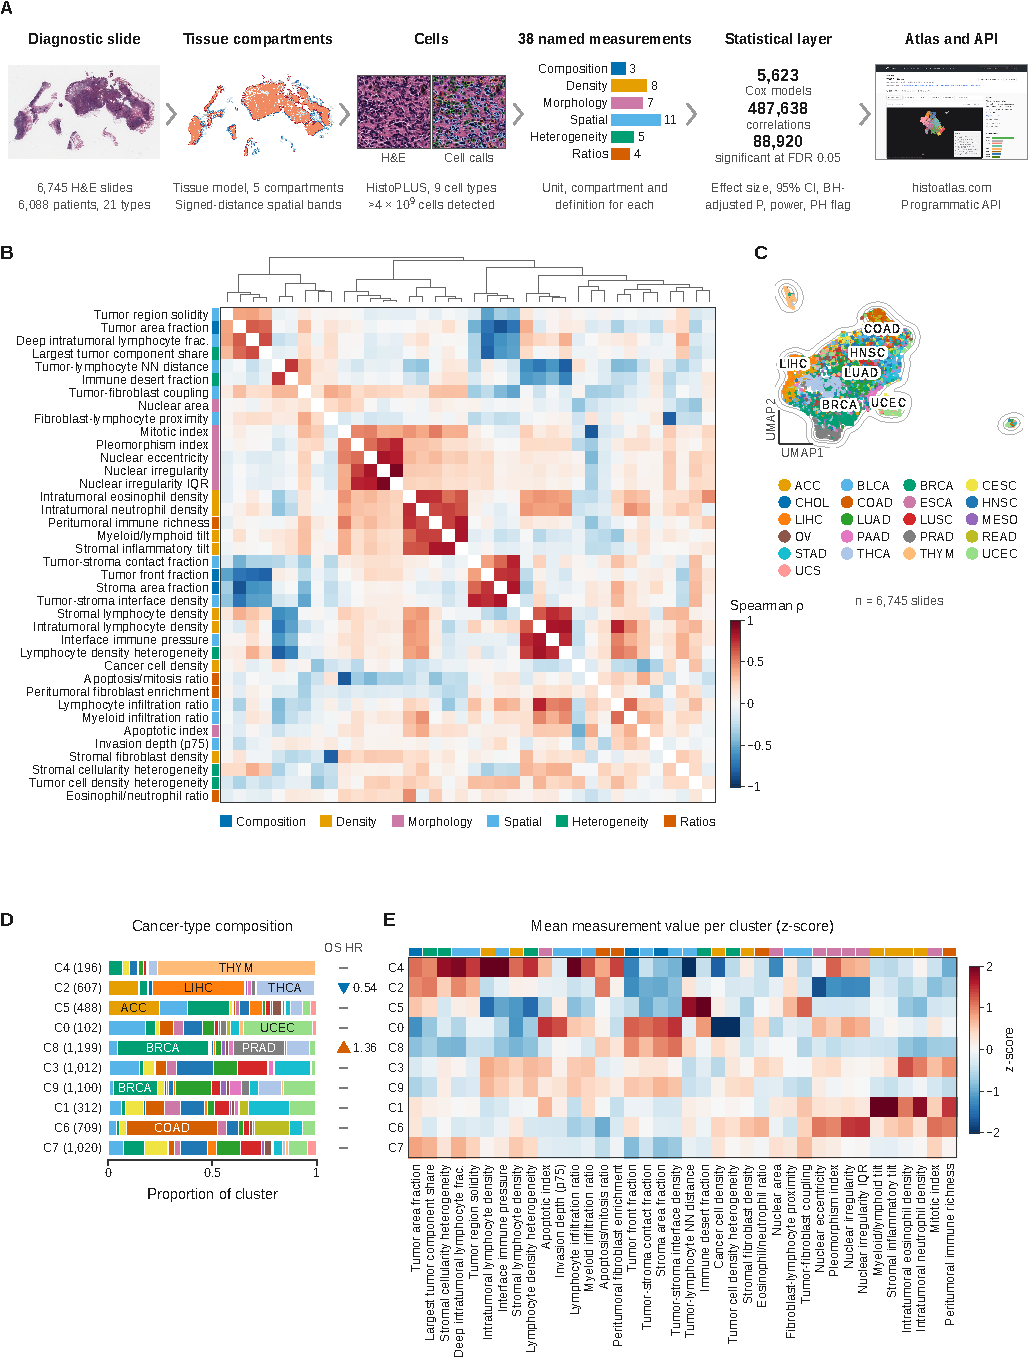
\includegraphics[width=\textwidth,height=0.92\textheight,keepaspectratio]{Figure1.pdf}\\[4pt]\textbf{Figure 1}\end{center}
\clearpage

\begin{center}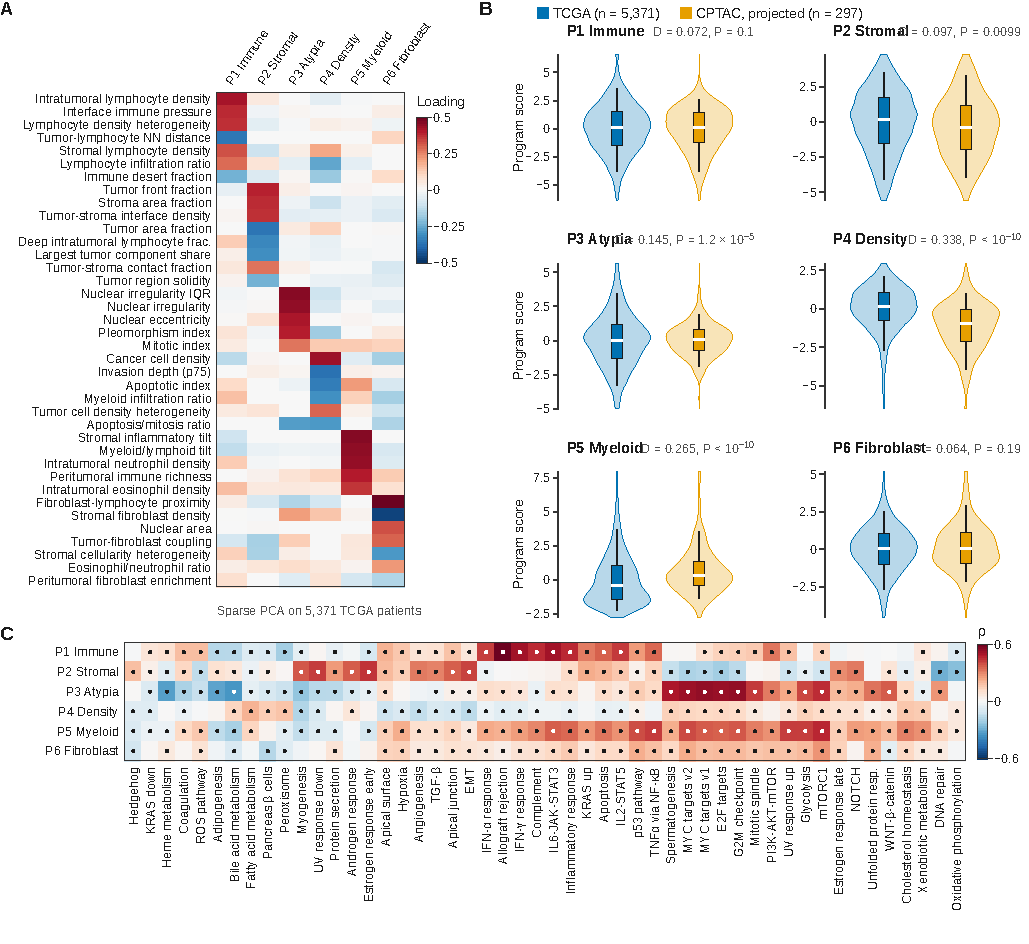
\includegraphics[width=\textwidth,height=0.92\textheight,keepaspectratio]{Figure2.pdf}\\[4pt]\textbf{Figure 2}\end{center}
\clearpage

\begin{center}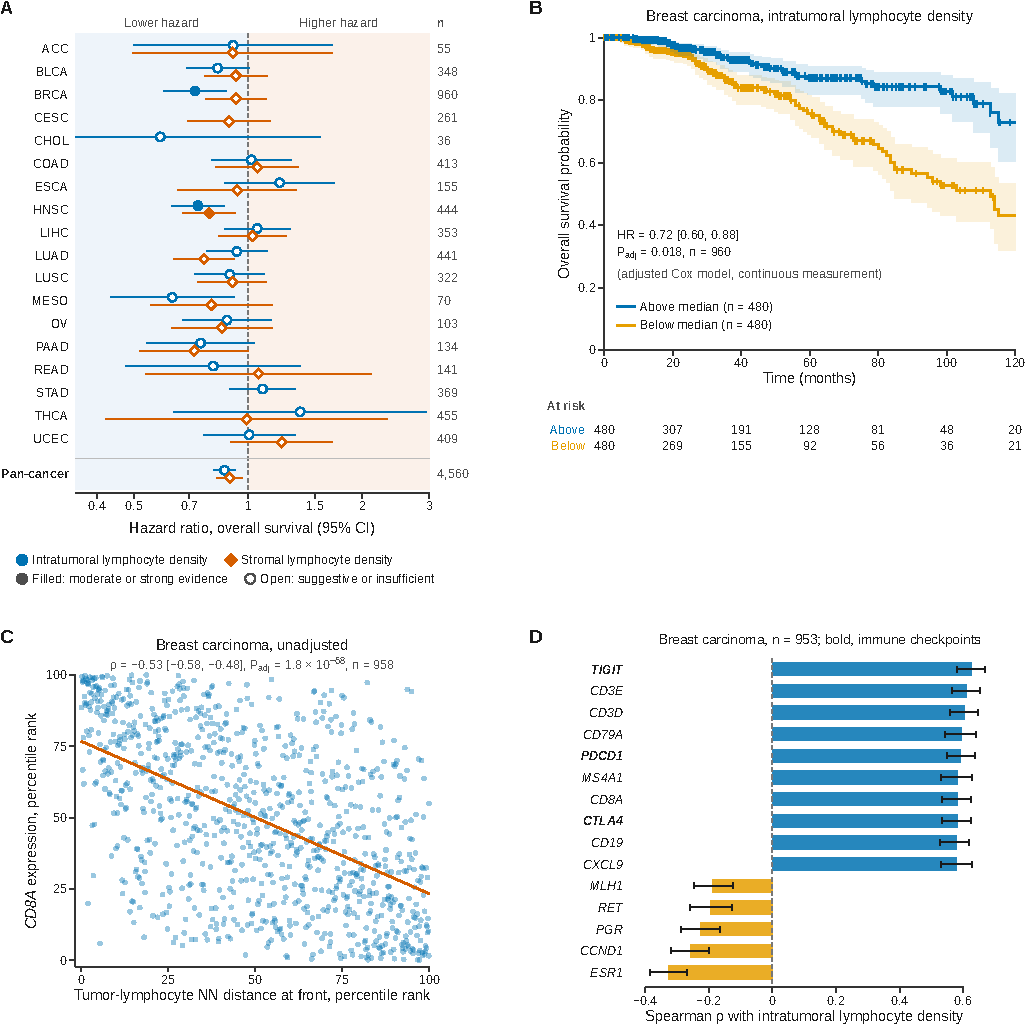
\includegraphics[width=\textwidth,height=0.92\textheight,keepaspectratio]{Figure3.pdf}\\[4pt]\textbf{Figure 3}\end{center}
\clearpage

\begin{center}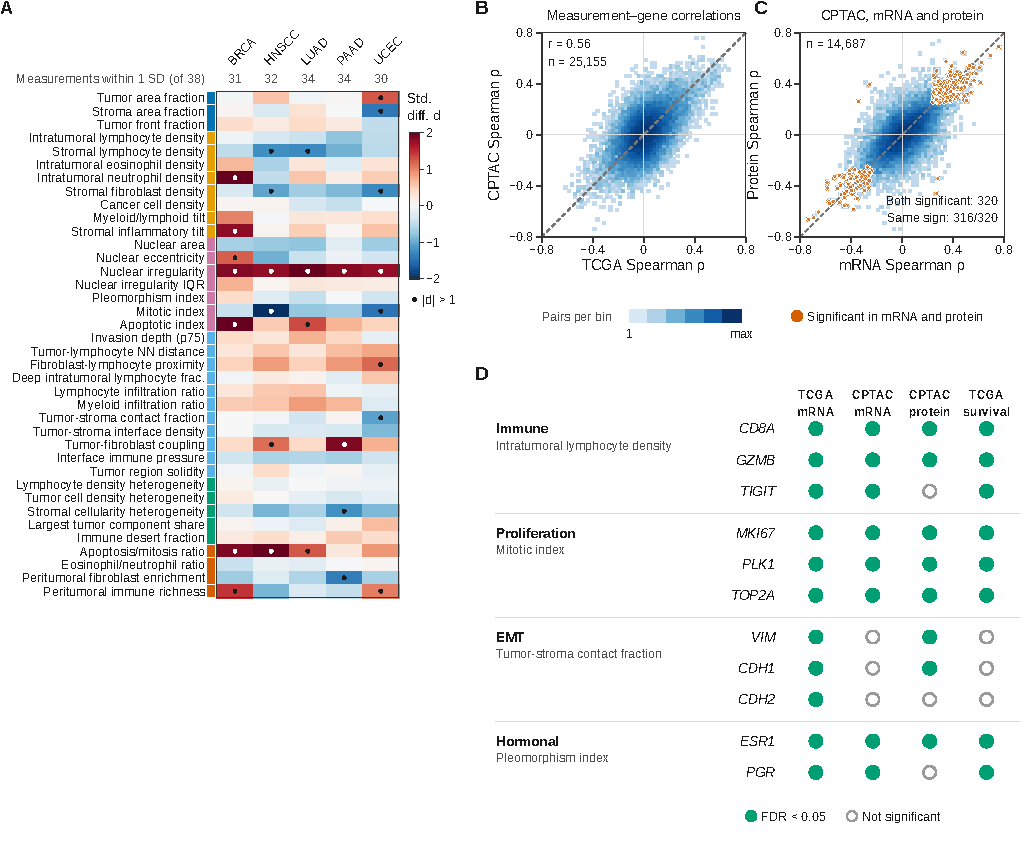
\includegraphics[width=\textwidth,height=0.92\textheight,keepaspectratio]{Figure4.pdf}\\[4pt]\textbf{Figure 4}\end{center}
\clearpage

\begin{center}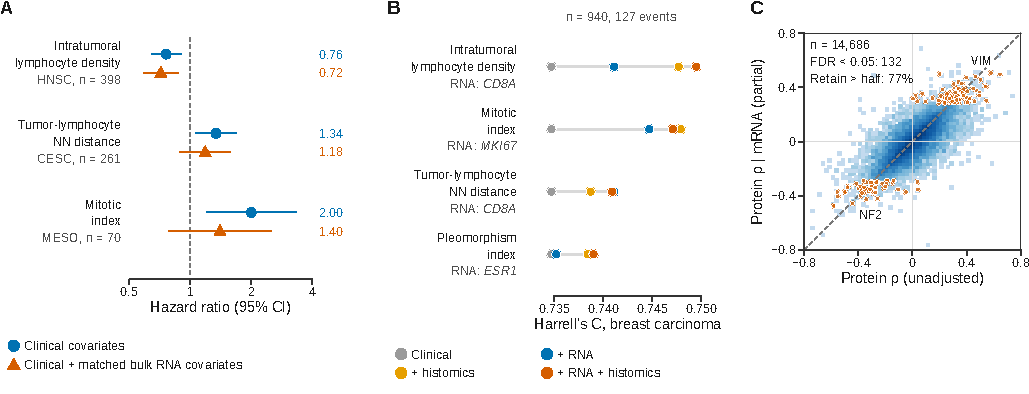
\includegraphics[width=\textwidth,height=0.92\textheight,keepaspectratio]{Figure5.pdf}\\[4pt]\textbf{Figure 5}\end{center}
\clearpage

\begin{center}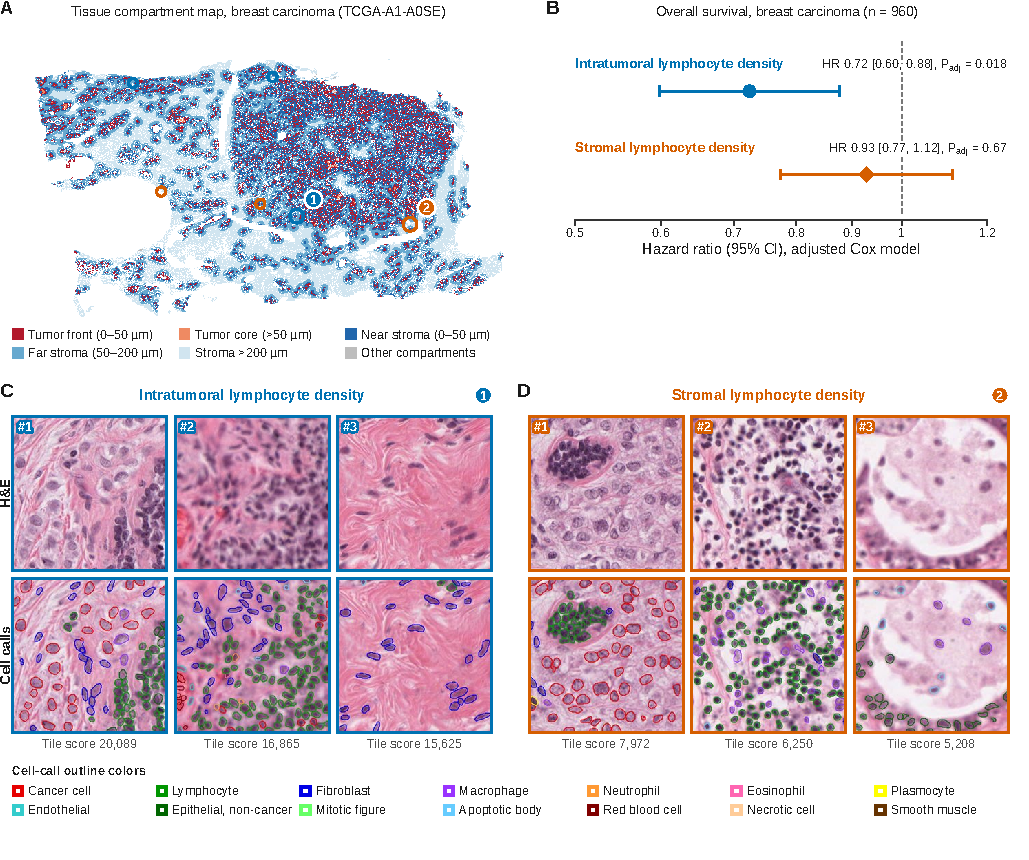
\includegraphics[width=\textwidth,height=0.92\textheight,keepaspectratio]{Figure6.pdf}\\[4pt]\textbf{Figure 6}\end{center}
\clearpage


\end{document}
